\sepframe{II. Reinforcement Learning Methods}

\begin{frame}
\frametitle{Latent structure via marginalization}
\begin{itemize}
    \item Given a sentence-label pair $(x, y)$ and its \textbf{known} parse
        tree $\z$,\\
        \uncover<2->{\quad we can make a prediction $\yhat(\z; x)$ \\}
        \uncover<3->{\quad and incur a loss,
        $$L(\yhat(\z; x), y) \uncover<4->{~\text{or simply}~L(\z)$$}}
    \item<5-> But we don't know $\z$!
    \item<6-> In this section: \\
        \quad we jointly learn a structured prediction model $\parser$\\
        \uncover<7->{\quad by optimizing the \textbf{expected loss}, \\
        $$ \EE_{\parser} \big[ L(\z) \big] $$}

\end{itemize}


\end{frame}

\sepframe[mygr]{But first, supervised SPINN}


\begin{frame}
\frametitle{\underline{S}tack-augmented \underline{P}arser-\underline{I}nterpreter \underline{N}eural-\underline{N}etwork}%
{\cornercite{bowman-spinn}}
\begin{figure}
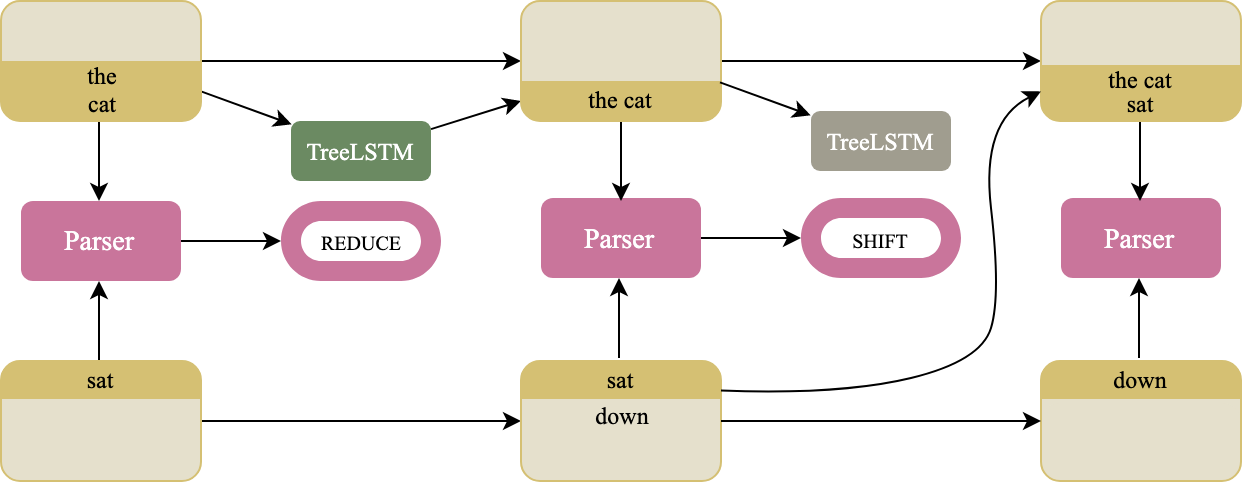
\includegraphics[width=0.8\textwidth]{img/spinnLatentTutorial.png}
\end{figure}
\end{frame}%


\begin{frame}%
\frametitle{\underline{S}tack-augmented \underline{P}arser-\underline{I}nterpreter \underline{N}eural-\underline{N}etwork}%
{\cornercite{bowman-spinn}}

\begin{itemize}%
\item Joint learning: Combines a constituency parser and a sentence representation model.
\item<2-> The parser, $f_{\parp}(x)$ is a transition-based \textbf{shift-reduce} parser. It looks at top two elements of stack and top element of the buffer.
\item<3-> \textbf{TreeLSTM} combines top two elements of the stack when the parser choses the {\rmfamily\scshape{reduce}} action.
\end{itemize}%
\end{frame}

\begin{frame}
\frametitle{\underline{S}tack-augmented \underline{P}arser-\underline{I}nterpreter \underline{N}eural-\underline{N}etwork}%
{\cornercite{bowman-spinn}}

\begin{figure}
\only<1>{\vspace{-1cm}\hspace*{1cm}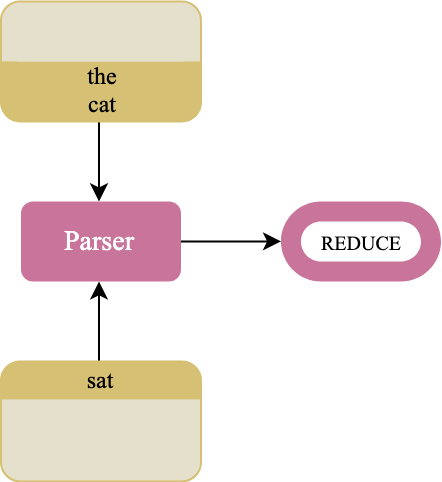
\includegraphics[width=0.3\textwidth,left]{img/200_spinn_1.png}}
\only<2>{\vspace{-1cm}\hspace*{1cm}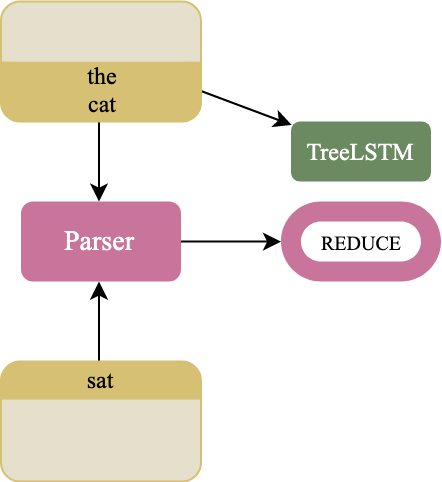
\includegraphics[width=0.3\textwidth,left]{img/200_spinn_2.png}}
\only<3>{\vspace{-1cm}\hspace*{1cm}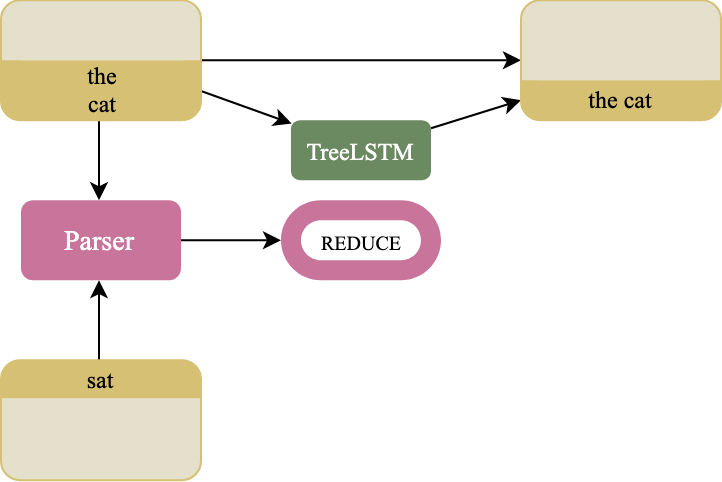
\includegraphics[width=0.5\textwidth,left]{img/200_spinn_3.png}}
\only<4>{\vspace{-1cm}\hspace*{1cm}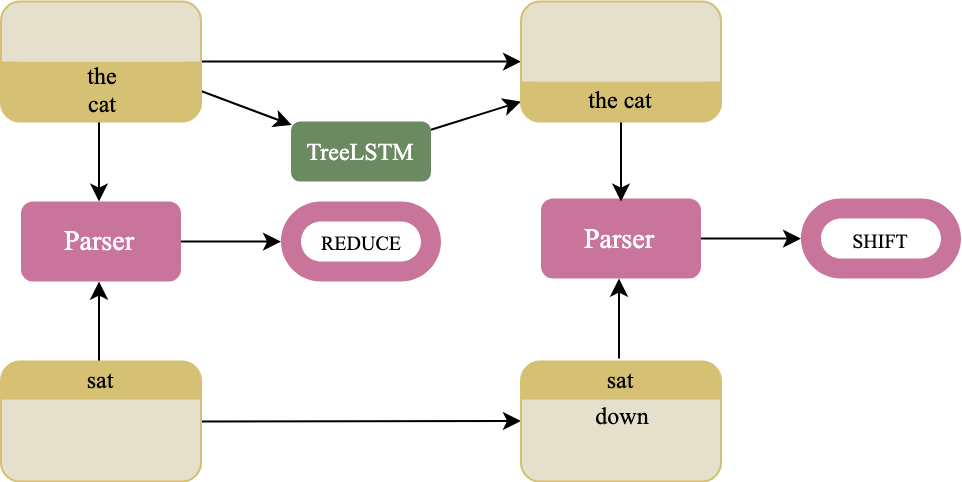
\includegraphics[width=0.65\textwidth,left]{img/200_spinn_4.png}}
\only<5>{\vspace{-1cm}\hspace*{1cm}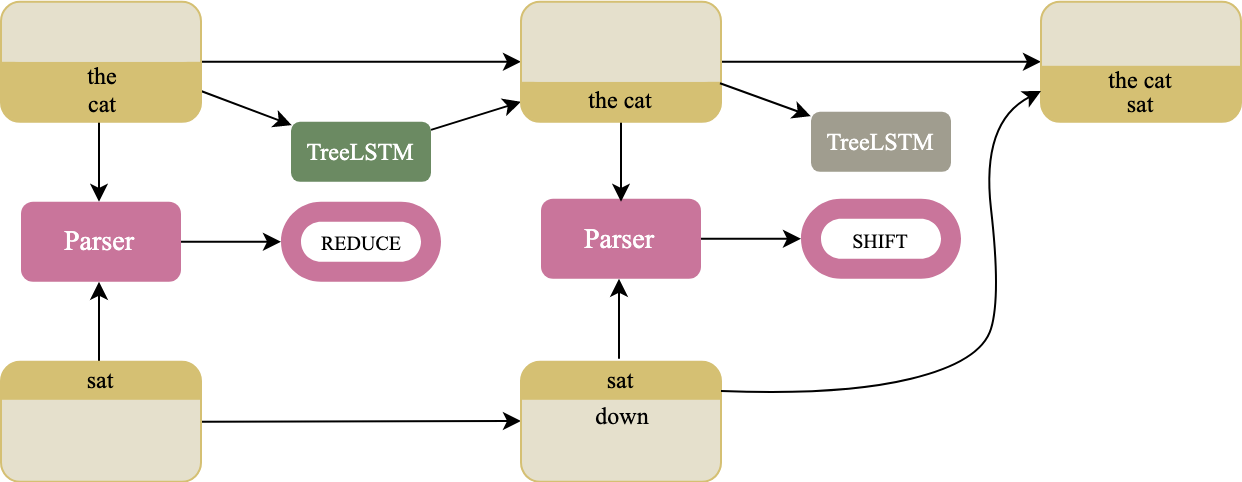
\includegraphics[width=0.8\textwidth,left]{img/200_spinn_5.png}}
\only<6>{\vspace{-1cm}\hspace*{1cm}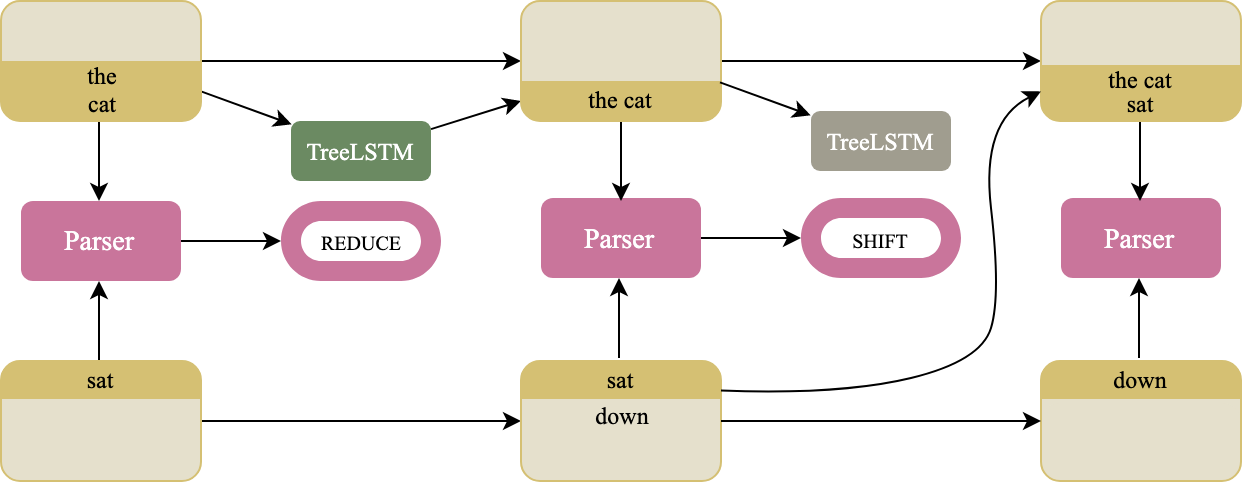
\includegraphics[width=0.8\textwidth,left]{img/spinnLatentTutorial.png}}
\end{figure}
\end{frame}%



%%% SR Math %%%
\begin{frame}
\frametitle{Shift-Reduce parsing}
\begin{itemize}
\item[] We can write a shift-reduce style parse as a sequence of Bernoulli random variables,
$$ \z = \{z_1, \ldots, z_{2L-1}\}$$
\item[] where, $z_j \in \{0,1\} \ \forall j\in[1,2L-1]$
\end{itemize}
\end{frame}

\begin{frame}
\frametitle{Shift-Reduce parsing}
\begin{itemize}
\item[] A sequence of Bernoulli trials but with conditional dependence,
$$p(z_1, z_2, \ldots, z_{2L-1}) = \displaystyle\prod_{j=1}^{2L-1} p(z_j \mid z_{<j})$$
\end{itemize}
\end{frame}




\begin{frame}
\frametitle{Latent structure learning with SPINN}

\begin{itemize}
\item<2-> But now, remove syntactic supervision from SPINN.
\item[] \begin{figure}
\centering
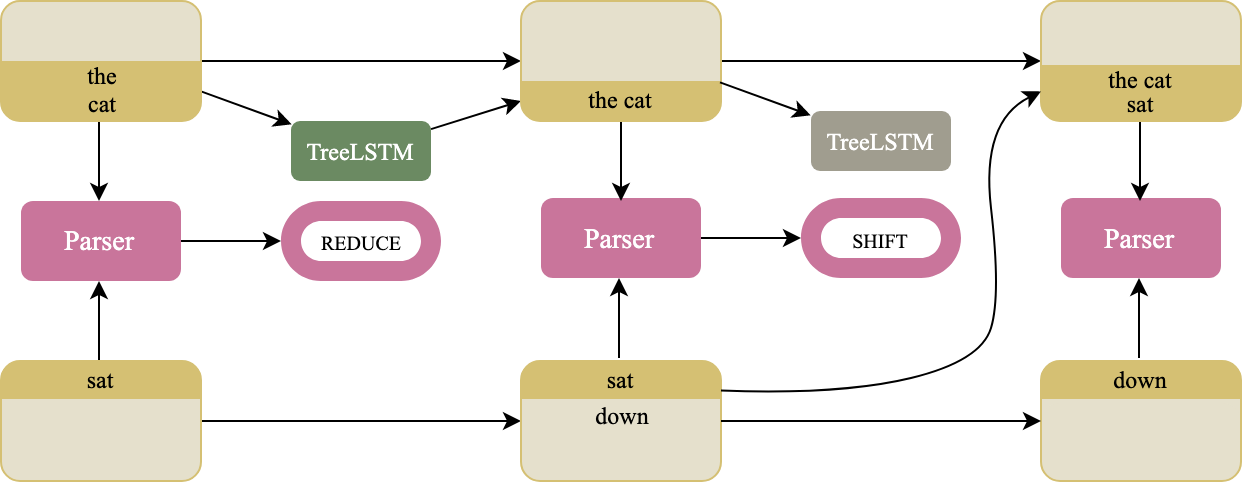
\includegraphics[width=0.6\textwidth]{img/spinnLatentTutorial.png}
\end{figure}
\item<3-> We model the parse, $\z$, as a latent variable with our parser
as the score function estimator, $f_{\parp}(x)$.
\item<4-> With shift-reduce parsing, we're making discrete decisions $\Rightarrow$ REINFORCE as a ``natural" solution.
\end{itemize}

\end{frame}


\sepframe[mygr]{Unsupervised SPINN}


\begin{frame}
\frametitle{Unsupervised SPINN}
\begin{itemize}
	\item[] No syntactic supervision.
	\item[] Only reward is from the downstream task.
	\item[] We only get this reward after parsing the full sentence.
\end{itemize}
\end{frame}

\begin{frame}
\frametitle{SPINN with REINFORCE}
{\cornercite{williams-reinforce}}

Some basic terminology,
\begin{itemize}
\item The \underline{action space} is $z_j\in \{${\rmfamily\scshape{shift}},{\rmfamily\scshape{reduce}}$\}$, and $\z$ is a sequence of actions.
\item<2-> Training parser network parameters, $\parp$ with REINFORCE
\item<3-> The \underline{state}, $\bs{h}$, is the top two elements of the stack and the top element of the buffer.
\item<4-> Learning a \underline{policy network} $\pi(\z \mid \bs{h}; \parp)$
\item<5-> Maximize the \underline{reward}, where $\mathcal{R}$ is performance on the downstream task like sentence classification.
\end{itemize}

\uncover<6>{\overlaybox{NOTE: Only a single reward at the end of parsing.}}

\end{frame}

%%% REINFORCE Algorithm %%%
\begin{frame}%
\frametitle{Through the looking glass of REINFORCE}%
%{\cornercite{williams-reinforce}}

\vspace{-.5\baselineskip}%
\begin{align*}
	\nabla_{\parp} \EE_{\z\sim \parser}[L(\z)] \uncover<2->{&= \nabla_{\parp}
\left[\sum_{\z} L(\z) \parser  \right] \\}
    \uncover<2->{&\small\textit{(By definition of expectation. How to evaluate?)}\\}
    \uncover<3->{&=\sum_{\z} L(\z) \nabla_{\parp} \parser \\}
    %\uncover<3->{&\small\textit{(Not an expectation!)}\\}
    \uncover<4->{&= \sum_{\z} L(\z) \parser \nabla_{\parp} \log \parser \\}
    \uncover<4->{&\small\textit{(By Leibniz integral rule for}\scriptscriptstyle\log\textit{)} \\}
    \uncover<5->{&= \EE_{\z \sim \parser}[L(\z) \nabla_{\parp} \log \parser]}
\end{align*}
\end{frame}




%%% Yogatama %%%
\begin{frame}
\frametitle{SPINN with REINFORCE, aka RL-SPINN}
\begin{itemize}
\item[]\cite{Yogatama2016LearningTC} uses REINFORCE to train SPINN!\\
\item<2->[] However, this vanilla implementation isn't very effective at learning syntax.
\item<3->[] This model fails to solve a simple toy problem.
\end{itemize}
\end{frame}



%%%% LISTOPS %%%%
\begin{frame}
\frametitle{Toy problem: ListOps}%
{\cornercite{nangia-listops}}

\begin{figure}[t]
\centering
\scalebox{1.2}{
\begin{forest}
 shape=coordinate,
 where n children=0{
   tier=word
 }{},
 nice empty nodes
[ [ [ [ [ [\textsc{[max}] [2] ] [9] ] [ [ [ [\textsc{[min}] [4] ] [7] ] [\textsc{]}] ] ] [0] ] [\textsc{]}] ]
\end{forest}
}
%\caption{\label{fig:exampletrees} Example of a parsed ListOps sequence. The parse is left-branching within each list, and each constituent is either a partial list, an integer, or the final closing bracket.}
\end{figure}
\end{frame}


\begin{frame}
\frametitle{Toy problem: ListOps}
{\cornercite{nangia-listops}}

\makebox[0.95\textwidth][c] {% two boxes
\begin{minipage}[t][][c]{.45\textwidth}

\begin{table}[t!]\small
\small \centering
\begin{tabular}{lcccc}
\toprule
 & \multicolumn{2}{c}{\bf Accuracy} & \bf Self  \\
\bf Model & \pmb{$\mu (\sigma)$} & \bf max & \bf F1 \\
\midrule
LSTM & 71.5 (1.5) & \bf 74.4 & - \\
RL-SPINN & 60.7 (2.6) & 64.8 & 30.8 \\
\midrule
Random Trees & - & - & 30.1\\
\bottomrule
\end{tabular}
%\caption{\label{tab:var} \textit{Accuracy} shows accuracy across four runs of the models (expressed as mean, standard deviation, and maximum). \textit{Self F1} shows how well each of these four model runs agrees in its parsing decisions with the other three.}
\end{table}

\end{minipage}%
\hfill%
%
%
\begin{minipage}[t][][c]{.5\textwidth}
\vspace{2.5cm}
\begin{table}[t!]
\small \centering
\begin{tabular}{lcccc}
\toprule
 & \multicolumn{3}{c}{\bf F1 wrt.} & \bf Avg.  \\
\bf Model & \bf LB & \bf RB & \bf GT & \bf Depth  \\
\midrule
48D~~ RL-SPINN &\bf  64.5 & \bf 16.0 & 32.1 & \bf 14.6 \\
128D RL-SPINN & 43.5 & 13.0 & \bf 71.1 & 10.4 \\
%\midrule
%48D~~ ST-Gumbel & 52.2 & 15.3 & 55.3 & 11.1 \\
%128D ST-Gumbel & 56.5 & 9.8 & 57.3 & 12.7 \\
\midrule
GT Trees & 41.6 & 8.8 & 100.0 & 9.6 \\
Random Trees & 24.0 & 24.0 & 24.2 & 5.2 \\
\bottomrule
\end{tabular}
%\caption{\label{tab:f1} \textit{F1 wrt.} shows F1 scores on ListOps with respect to left-branching (LB), right-branching (RB), and ground-truth (GT) trees. \textit{Avg. Depth} shows the average across sentences of the average depth of each token in its tree.}
\end{table}

\end{minipage}}

\uncover<2>{\overlaybox{But why?}}

\end{frame}




%%%% PROBLEMS %%%%
\begin{frame}
\frametitle{RL-SPINN's Troubles}
\begin{itemize}
\item[] This system faces at least two big problems,
\begin{itemize}
\item<2->[] {\large 1. High variance of gradients}
\item<2->[] {\large 2. Coadaptation}
\end{itemize}
\end{itemize}
\end{frame}


%%%% VARIANCE %%%%
\begin{frame}
\frametitle{High variance}

\begin{itemize}
\item We have a single reward at the end of parsing.
\item<2-> We are sampling parses from very large search space!\\ \textbf{Catalan number} of binary trees.
\only<3>{
	\begin{align*}
		3 \text{ tokens } &\Rightarrow 5 \text{ trees} \\
		5 \text{ tokens } &\Rightarrow 42 \text{ trees} \\
		10 \text{ tokens } &\Rightarrow 16796 \text{ trees}
	\end{align*}
}
\item<4-> And the policy is stochastic.
\end{itemize}
\end{frame}


\begin{frame}
\frametitle{High variance}

\begin{itemize}
\item[]<1>{So, sometimes the policy lands in a ``rewarding state":}\\
\end{itemize}

\only<1>{\begin{figure}[t]
\centering
	\scalebox{1.0}{
	\begin{forest}
		shape=coordinate,
		where n children=0{
			tier=word
		}{},
		nice empty nodes
		[ [ [ [ [ [\textsc{[sm}] [\textsc{[sm}] ] [\textsc{[sm}] ] [ [ [\textsc{[max}] [ [5] [ [6] [\textsc{]}] ] ] ] [ [2] [\textsc{]}] ] ] ] [ [0] [ [\textsc{]}] [ [5] [ [0] [8] ] ] ] ] ] [ [6] [\textsc{]}] ] ]
	\end{forest}
}
\caption{Truth: 7; Pred: 7}
\end{figure}
}

\begin{itemize}
\item[]<2>{Sometimes it doesn't:}
\end{itemize}

\only<2>{\begin{figure}[t]
\centering
	\scalebox{1.0}{
	\begin{forest}
		shape=coordinate,
		where n children=0{
			tier=word
		}{},
		nice empty nodes
		[ [ [ [ [ [ [ [ [ [ [ [ [\textsc{[max}] [ [\textsc{[med}] [ [\textsc{[med}] [1] ] ] ] [\textsc{[sm}] ] [3] ] [1] ] [3] ] [\textsc{]}] ] [9] ] [\textsc{]}] ] [6] ] [\textsc{]}] ] [5] ] [\textsc{]}] ]
	\end{forest}
}
\caption{Truth: 6; Pred: 5}
\end{figure}
}

\end{frame}


\begin{frame}
\frametitle{High variance}
\begin{itemize}
\item[] \textbf{Catalan number} of parses means we need many many samples to lower variance!
\item<2->[] Possible solutions,
\begin{itemize}
\item[] 1. Gradient normalization
\item[] 2. Control variates, aka baselines
\end{itemize}
\end{itemize}
\end{frame}


%%% CONTROL VARIATES %%%
\begin{frame}
\frametitle{Control variates}
\begin{itemize}
\item A simple control variate: moving average of recent rewards
\item<2-> Parameters are updated using the \underline{advantage} which is the difference between the reward, $\mathcal{R}$, and the baseline prediction.
\item[]<3-> So,
\begin{align*}
	\nabla \EE_{\z\sim\pi(\z)} = \EE_{\z\sim \pi(\z)}[\left(\textcolor{tBleu}{L(\z)} - \textcolor{tPink}{b(\bs{x})}\right) \nabla \pi(\z)]
\end{align*}
\item[]<4->Which we can do because,
\begin{align*}
	\sum_z \textcolor{tPink}{b(\bs{x})} \nabla\pi(\z) = \textcolor{tPink}{b(\bs{x})}\sum_z\nabla\pi(\z) = \textcolor{tPink}{b(\bs{x})} \nabla 1 = 0
\end{align*}
\end{itemize}
\end{frame}


%%%% PROBLEMS %%%%
\begin{frame}
\frametitle{Issues with SPINN with REINFORCE}
\begin{itemize}
\item[] This system faces two big problems,
\begin{itemize}
\item[] {\large 1. High variance of gradients}
\item[] {\large 2. Coadaptation}
\end{itemize}
\end{itemize}
\end{frame}


%%% COADAPTATION %%%
\begin{frame}
\frametitle{Coadaptation problem}
\begin{itemize}
\item[] Learning composition function parameters $\clfp$ with backpropagation,
\item[] and parser parameters $\parp$ with REINFORCE.
\item<2->[]
\item<2->[] Generally, $\clfp$ will be learned more quickly than $\parp$,
 \item<2->[] making it harder to explore the parsing search space and optimize for $\parp$.
\item<3->[]
\item<3->[] Difference in variance of two gradient estimates.
\end{itemize}
\uncover<4>{\overlaybox{Possible solution:\\ Proximal Policy Optimization (Schulman et al., 2017)}}
\end{frame}


\begin{frame}
\frametitle{Making REINFORCE+SPINN work}
\begin{itemize}
\item[] \cite{havrylov-2019-cooperative} use,
	\begin{itemize}
		\item[] 1. Input dependent control variate
		\item[] 2. Gradient normalization
		\item[] 3. Proximal Policy Optimization
	\end{itemize}
\item<2->[]
\item<2->[] They solve ListOps!
\item<3->[] However, does not learn English grammars.
\end{itemize}
\end{frame}



\begin{frame}%
\frametitle{Should I? Shouldn't I?}%
\makebox[\textwidth][c] {% two boxes
\begin{minipage}[t][][c]{.45\textwidth}
\begin{itemize}
\item Unbiased!
\item<3-> In a simple setting, with enough tricks, it can work! \emoji{happ}
\end{itemize}
\end{minipage}

\begin{minipage}[t][][c]{.45\textwidth}
\begin{itemize}
\item<2-> High variance \emoji{frown}
\item<4-> Has not yet been very effective at learning English syntax.
\end{itemize}
\end{minipage}

}
\end{frame}
